\section{Dinâmica orbital}
\label{sec_dinamica_orbital}

O problema de dois-corpos na mecânica celeste descreve o movimento de duas massas pontuais que interagem exclusivamente pela atração gravitacional mútua, conforme as leis de Newton.
Quando a massa de um dos corpos é significativamente superior à do outro, o sistema pode ser simplificado para o movimento de um corpo em torno de um primário, configuração conhecida como problema de corpo central.
Essa formulação constitui a base da dinâmica orbital de espaçonaves em torno de planetas.

No contexto de missões de encontro e acoplamento (\gls{rvdb}), o problema restrito de dois corpos fornece o fundamento para a descrição do movimento relativo entre duas espaçonaves em órbita terrestre, servindo de base para o desenvolvimento de modelos mais específicos, como as equações de \gls{hcw}.
% Por outro lado, o problema geral, sem restrição quanto à magnitude das massas, descreve o movimento de ambos os corpos em torno de um \gls{cdm} comum, resultando em trajetórias que seguem as seções cônicas (elipse, parábola ou hipérbole), detalhadas na subseção~\ref{sec_conicas}.
A Lei da Gravitação Universal de Newton é, portanto, o alicerce fundamental tanto da mecânica celeste quanto da astrodinâmica moderna.


\subsection{O problema de dois-corpos: Movimento absoluto e relativo}
\label{sec_doiscorpos}

Nesta seção, considera-se o problema dinâmico de duas massas pontuais sob a influência de sua atração gravitacional mútua, denominado em mecânica celeste como o problema dos dois corpos. A partir das leis do movimento e da Lei da Gravitação Universal de Newton, o problema é formulado para verificar as três leis empíricas de Kepler \cite{vallado2007fundamentals} sobre o movimento planetário, enunciadas a seguir:

\begin{itemize}
    \item Os planetas giram em torno do Sol em órbitas elípticas, com o Sol em um dos focos (Lei das Órbitas).
    \item O segmento (raio vetor) que une o Sol a um planeta varre áreas iguais em intervalos de tempo iguais (Lei das Áreas).
    \item O quadrado do período orbital de um planeta é diretamente proporcional ao cubo
de sua distância média ao Sol (Lei dos Períodos)\cite{SaraivaKeplerAula}.
\end{itemize}

Essas leis foram deduzidas inicialmente por Kepler a partir da análise de dados observacionais coletados por Tycho Brahe.
A grande contribuição de Isaac Newton foi fornecer a formulação matemática consistente que explicou a causa física desse movimento.
Enquanto Kepler constatou o comportamento dos planetas empiricamente, Newton demonstrou, por meio da Lei da Gravitação Universal, o motivo pelo qual os planetas seguem tais órbitas.
No problema dos dois corpos, ilustrado na Figura~\ref{fig_two_body_general}, dois corpos massivos interagem pela atração gravitacional mútua e movem-se em relação a um sistema inercial.
Matematicamente:

\begin{equation}
\label{eq_wie3_1}
m_1 \ddot{\vec R}_1 =
+\, G \frac{m_1 m_2}{r^3}\, \vec r,
\end{equation}

\begin{equation}
\label{eq_wie3_2}
m_2 \ddot{\vec R}_2 =
-\, G \frac{m_1 m_2}{r^3}\, \vec r.
\end{equation}

Em que $m_1$ e $m_2$ são as massas dos corpos $1$ e $2$, respectivamente; $G$ é a constante gravitacional universal; $\vec R_1$ e $\vec R_2$ são os vetores posição (no referencial inercial) dos corpos $m_1$ e $m_2$; $\ddot{\vec R}_1$ e $\ddot{\vec R}_2$ são suas acelerações inerciais; e $\vec r$ é o vetor posição relativa definido por:

\begin{equation}
\label{eq_vetor_posicao_r}
\vec r = \vec R_{\,2} - \vec R_{\,1}.
\end{equation}

Além disso, define-se a distância relativa (módulo do vetor relativo) como:

\begin{equation}
\label{eq_norma_r}
r \triangleq \|\vec r\|.
\end{equation}

A equação \eqref{eq_vetor_posicao_r} define o vetor posição relativa de $m_2$ em relação a $m_1$.
A Figura~\ref{fig_two_body_general} ilustra o problema de dois-corpos em relação ao sistema inercial.

\begin{figure}[H]
\centering
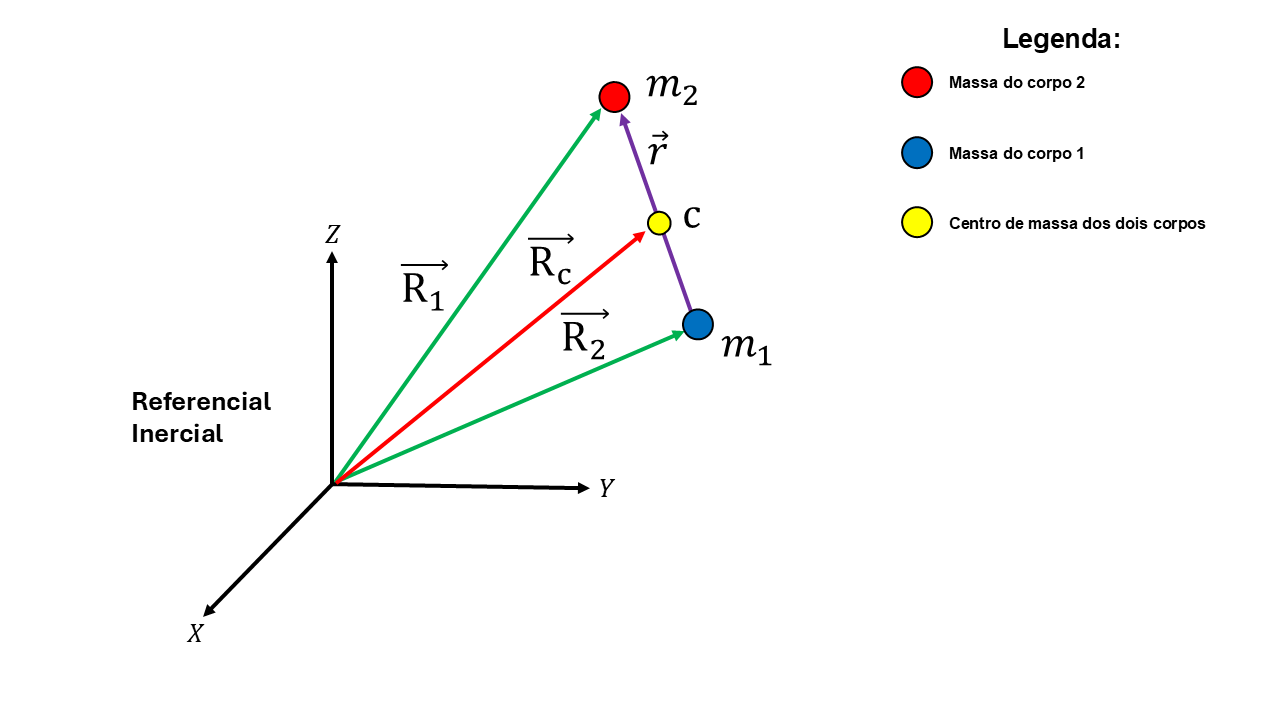
\includegraphics[width=1\linewidth]{4 Formulacao matematica/Imagens/Fig_3_1_Wie.png}
\caption{Problema de dois-corpos.}
\label{fig_two_body_general}
\end{figure}

Portanto, somando as equações \eqref{eq_wie3_1} e \eqref{eq_wie3_2}, obtém-se:
\begin{equation}
\label{eq_somaAceleracao_Corpo1e2}
m_1 \ddot{\vec R}_1 + m_2 \ddot{\vec R}_2 = \vec 0.
\end{equation}

Pela definição do \gls{cdm}, como explica \cite{halliday_resnick_walker_fundamentos1}, para um sistema discreto com duas partículas, a posição do centro de massa $\vec{R}_c$ é tal que a soma dos momentos de massa em relação a ele seja nula. Matematicamente:

\begin{equation}
m_1\left(\vec R_1-\vec R_{c}\right)+m_2\left(\vec R_2-\vec R_{c}\right)=\vec 0.
\label{eq_def_cm_duas_particulas}
\end{equation}

O termo $\vec{R}_c$ é o vetor posição do centro de massa do sistema $(m_1, m_2)$ em relação à origem do referencial inercial.
Reorganizando \eqref{eq_def_cm_duas_particulas}, isola-se $\vec{R}_c$ como a média ponderada das posições das massas:

\begin{equation}
(m_1+m_2)\,\vec R_{c} = m_1\,\vec R_1 + m_2\,\vec R_2,
\end{equation}

e, portanto, obtém-se a definição do \gls{cdm} dos dois corpos:

\begin{equation}
\vec R_{c} = \frac{m_1\,\vec R_1 + m_2\,\vec R_2}{m_1+m_2}.
\label{eq_Rc_cm_duas_particulas}
\end{equation}

Tomando duas derivadas temporais de \eqref{eq_Rc_cm_duas_particulas}, com massas constantes, resulta
\begin{equation}
(m_1+m_2)\,\ddot{\vec R}_{c} = m_1\,\ddot{\vec R}_1 + m_2\,\ddot{\vec R}_2.
\label{eq_Rc_ddot_relacao}
\end{equation}

Usando \eqref{eq_somaAceleracao_Corpo1e2} em \eqref{eq_Rc_ddot_relacao}, conclui-se que

\begin{equation}
\label{eq_Rc_vec0}
\ddot{\vec R}_{c} = \vec 0 \implies \dot{\vec{R}}_{c} = \text{constante}.
\end{equation}

Esse resultado implica que o \gls{cdm} dos dois corpos está em movimento uniforme ou é estacionário.

%%%%%%%%%%%%%%%%%%%%%%%%%%%%%%%%%%%%%%%

A condição \eqref{eq_Rc_vec0} não implica $\vec R_c(t)=\vec 0$, mas que o \gls{cdm} possui movimento retilíneo uniforme no referencial inercial. Integrando, obtém-se

\begin{equation}
\dot{\vec{R}}_{c}(t) = \dot{\vec{R}}_{c}(0),
\label{eq_Rc_dot_constante}
\end{equation}

\begin{equation}
\vec{R}_{c}(t) = \vec{R}_{c}(0) + \dot{\vec{R}}_{c}(0)\,t.
\label{eq_Rc_movimento_uniforme}
\end{equation}

O termo $\vec{R}_{c}(0)$ e $\dot{\vec{R}}_{c}(0)$ representam, respectivamente, a posição e a velocidade iniciais do \gls{cdm} mútuto de $m_1$ e $m_2$.
% no instante $t = 0$. Ainda, pode-se escolher a origem do referencial inercial no centro de massa no instante inicial, isto é, $\vec R_c(0)=\vec 0$. Além disso, escolhendo um referencial inercial no qual o centro de massa esteja em repouso no instante inicial, $\dot{\vec R}_c(0)=\vec 0$, a equação \eqref{eq_Rc_movimento_uniforme} reduz-se a

% \begin{equation}
% \vec R_c(t)=\vec 0.
% \label{eq_Rc_zero_por_escolha_referencial}
% \end{equation}


%%%%%%%%%%%%%%%%%%%%%%%%%%%%%%%%%%%%%%%%
Assim, metade dos 12 estados do sistema dinâmico foi resolvida ao descrever o movimento do \gls{cdm}.
Os 12 estados correspondem às posições e velocidades inerciais de ambos os corpos, isto é, $\vec R_1,\dot{\vec R}_1,\vec R_2,\dot{\vec R}_2$.
A dinâmica do \gls{cdm} determina 6 estados globais associados a $\vec R_c(t)$ e $\dot{\vec R}_c(t)$.
Os seis estados restantes estão associados ao movimento relativo entre as massas e podem ser obtidos por meio de
\begin{equation}
\vec r(t)=\vec R_2(t)-\vec R_1(t),
\label{eq_posicao_relativa}
\end{equation}
e
\begin{equation}
\dot{\vec r}(t)=\dot{\vec R}_2(t)-\dot{\vec R}_1(t).
\label{eq_velocidade_relativa}
\end{equation}

%%%%%%%%%%%%%%%%%%%%%%%%%%%%%%%%%%%%%%%%
Subtraindo a \eqref{eq_wie3_1} multiplicada por $m_2$ da \eqref{eq_wie3_2} multiplicada por $m_1$, obtém-se

\begin{equation}
m_1 m_2\left(\ddot{\vec R}_2-\ddot{\vec R}_1\right)
=
-\,G\,m_1 m_2\left(m_1+m_2\right)\frac{\vec r}{r^3}.
\end{equation}

O termo $\vec r\triangleq \vec R_2-\vec R_1$ e $r\triangleq\|\vec r\|$.

%%%%%%%%%%%%%%%%%%%%%%%%%%%%%%
Dividindo por $m_1 m_2$ e definindo

\begin{equation}
\mu \triangleq G(m_1+m_2),
\end{equation}

resulta
\begin{equation}
\label{eq_eqFundamentalDoisCorpos1}
\ddot{\vec{r}} + \mu\,\frac{\vec{r}}{r^3} = \vec 0,
\end{equation}

sendo reescrito como
\begin{equation}
\label{eq_eqFundamentalDoisCorpos}
\ddot{\vec r} = -\frac{\mu}{r^3}\,\vec r.
\end{equation}

O termo $\ddot{\vec r}$ é a aceleração inercial de $m_2$ em relação a $m_1$, e $\mu$ é o parâmetro gravitacional do sistema de dois corpos.
A equação \eqref{eq_eqFundamentalDoisCorpos} corresponde à forma vetorial fundamental do problema dos dois corpos \cite{wie2008space}.
Nesta etapa, $\mu=G(m_1+m_2)$ e as grandezas $\vec R_1$, $\vec R_2$ e $\vec r$ são definidas no referencial inercial.

%%%%%%%%%%%%%%%%%%%%%%%%%%%%%%%%%%%%%%%%%%%%
A partir de \eqref{eq_eqFundamentalDoisCorpos}, conforme \cite{wie2008space}, obtém-se o integral de energia tomando o produto escalar com $\dot{\vec r}$,

\begin{equation}
\ddot{\vec r}\cdot \dot{\vec r}
=
-\frac{\mu}{r^3}\,\vec r\cdot \dot{\vec r}
\label{eq_energia_dot_1}
\end{equation}

Observa-se que
\begin{equation}
\ddot{\vec r}\cdot \dot{\vec r}
=
\frac{1}{2}\frac{d}{dt}\!\left(\dot{\vec r}\cdot \dot{\vec r}\right),
\label{eq_identidade_ddotr_dotr}
\end{equation}

\begin{equation}
\frac{d}{dt}\!\left(\frac{1}{r}\right)
=
-\frac{1}{r^3}\,\vec r\cdot \dot{\vec r}.
\label{eq_identidade_d1sobrer}
\end{equation}

Definindo $v = \|\dot{\vec{r}}\|$ como o módulo da velocidade relativa, e substituindo as identidades em \eqref{eq_energia_dot_1}, tem-se:

\begin{equation}
\frac{d}{dt}\left(\frac{v^2}{2}-\frac{\mu}{r}\right)=0.
\label{eq_energia_constante}
\end{equation}

Isso implica que a quantidade entre parênteses é conservada, ou seja:

\begin{equation}
\frac{v^2}{2}-\frac{\mu}{r}=\mathcal{E}.
\label{eq_energia_especifica}
\end{equation}

% O termo $\mathcal{E}$ é constante e representa a energia mecânica específica do movimento relativo \cite{wie2008space} entre as duas espaçonaves.
O termo $\mathcal{E}$ é constante e representa a energia mecânica específica do movimento relativo \cite{wie2008space} entre as duas massas pontuais.
Com isso, obtém-se a equação vis-viva, que relaciona a velocidade $v$, a distância radial $r$ e o semieixo maior $a$ \cite{wie2008space}:

\begin{equation}
\label{eq_vis_viva}
v^2 = \mu\left(\frac{2}{r}-\frac{1}{a}\right).
\end{equation}

%%%%%%%%%%%%%%%% CONICAS
% \subsection{Características geométricas das seções cônicas}
% \label{sec_conicas}
% As características geométricas das seções cônicas, são fundamentais na mecânica orbital.
% A equação de uma seção cônica geral em termos de coordenadas polares $(r, \theta)$ é dada por \cite{wie2008space}:

% \begin{equation}
% \label{eq_conica_geral_polar}
% r = \frac{p}{1 + e \cos \theta}.
% \end{equation}

% O termo $p$ é o parâmetro geométrico ou \textit{semilatus rectum}, e $e$ é a excentricidade. O tamanho da seção cônica é determinado por $p$, enquanto sua forma é determinada por $e$.
% Sendo que, nessa parametrização, $\theta$ é a anomalia verdadeira medida a partir do periapsis; assim, para $\theta=\pm 90^\circ$ obtém-se $r=p$.
% A Figura~\ref{fig:conicas_wie} ilustra os elementos geométricos para os dois casos principais: (a) Elipse, sendo $0 \le e < 1$, e (b) Hipérbole, e o termo $e > 1$.

% \begin{figure}[H]
% \centering
% % Figura A - Elipse
% 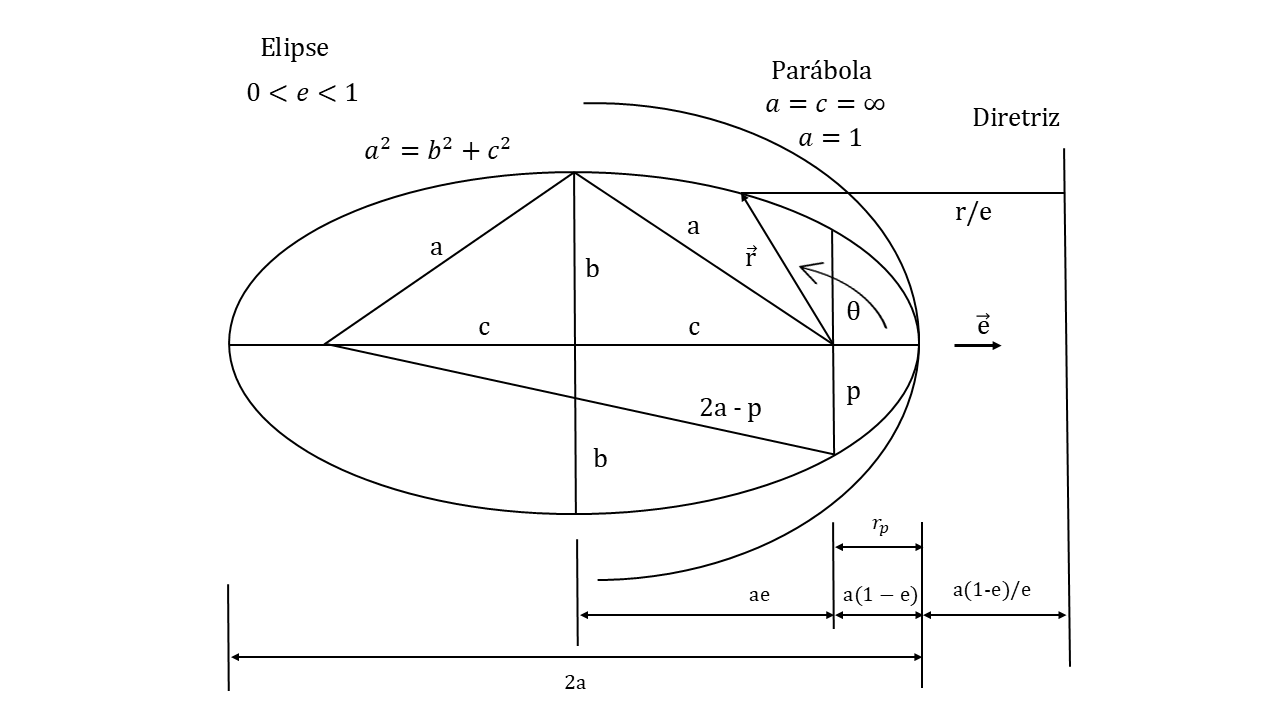
\includegraphics[width=0.85\linewidth]{4 Formulacao matematica/Imagens/Fig_3_3_a.png}
% \centerline{(a) Elipse ($0 < e < 1$)}
% \vspace{0.5cm} % Espaço entre as figuras

% % Figura B - Hipérbole
% 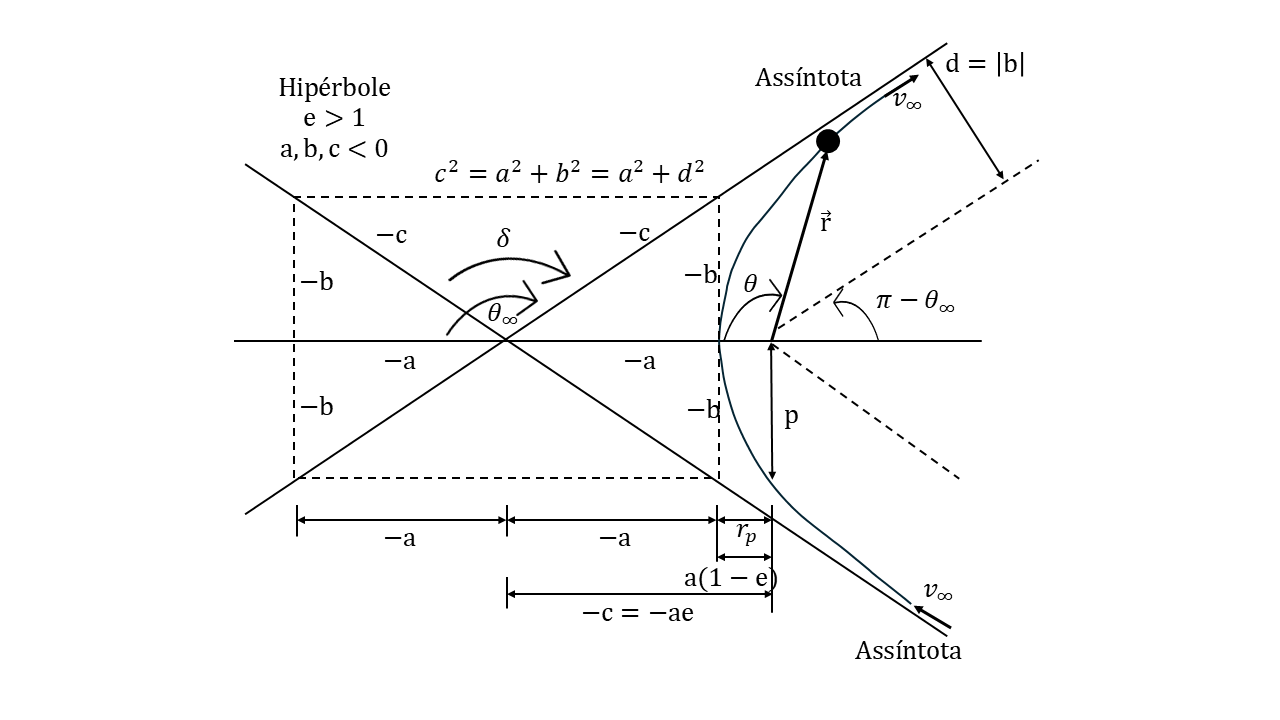
\includegraphics[width=0.85\linewidth]{4 Formulacao matematica/Imagens/Fig_3_3_b.png}
% \centerline{(b) Hipérbole ($e > 1$)}

% \caption{Características geométricas das seções cônicas.}
% \label{fig:conicas_wie}
% \end{figure}

% Para a elipse, a excentricidade é definida como $e = c/a$, por sua vez, $a$ é o semieixo maior e $c$ é a distância do centro geométrico ao foco principal. O parâmetro $p$ relaciona-se com $a$ e $e$ por \cite{wie2008space}:

% \begin{equation}
% \label{eq_parametro_p_elipse}
% p = a(1 - e^2).
% \end{equation}

% Os pontos da órbita mais próximo e mais distante do foco atrator são denominados, respectivamente, periapsis e apoapsis. As distâncias de periapsis ($r_p$) e apoapsis ($r_a$) são obtidas por:

% \begin{equation}
% r_p = a(1 - e),
% \end{equation}
% \begin{equation}
% r_a = a(1 + e).
% \end{equation}

% Já o semieixo menor $b$ relaciona-se com o semieixo maior através da identidade geométrica $a^2 = b^2 + c^2$, resultando em:
% \begin{equation}
% b = a\sqrt{1 - e^2}.
% \end{equation}

% No caso da hipérbole ($e > 1$), utilizada em manobras de sobrevoo ou escape, o semieixo maior $a$ é frequentemente tratado como negativo ($a < 0$) na convenção de energia, e o semieixo menor pode ser expresso por $b = |a|\sqrt{e^2 - 1}$.


%%%%%%%%%%%%%%%%%
\section{Equações do Movimento Orbital e Manobras Associadas ao Problema de RVD/B}

Nesta dissertação, a modelagem orbital do problema de \gls{rvdb} é formulada no contexto do problema restrito de dois corpos, assumindo-se que a massa do corpo primário é muito maior que a massa de cada espaçonave, isto é, $m_1 \gg m_2$. Nesse caso, o movimento orbital de cada veículo espacial pode ser descrito, com boa aproximação, como o movimento de um corpo de massa desprezível em torno do primário, que neste trabalho é a Terra.

Assim, o alvo e o perseguidor não são tratados como um sistema de dois corpos massivos girando em torno de um centro de massa comum, nem se considera a atração gravitacional mútua entre as duas espaçonaves. Cada veículo está sujeito predominantemente ao campo gravitacional da Terra e evolui em sua própria órbita geocêntrica. Desse modo, o movimento relativo relevante para missões de \gls{rvdb} é obtido pela diferença entre as órbitas do alvo e do perseguidor em torno do mesmo corpo primário.

Adota-se o referencial inercial geocêntrico para a propagação orbital e distinguem-se as variáveis do alvo e do perseguidor pelos subscritos $a$ e $p$, respectivamente. Os vetores $\vec r_a$ e $\vec r_p$ denotam as posições inerciais do alvo e do perseguidor em relação ao centro da Terra, com $r_a=\|\vec r_a\|$ e $r_p=\|\vec r_p\|$. A força $\vec F$ representa uma força não gravitacional aplicada ao perseguidor, como a força de controle produzida pelo sistema propulsivo.

No problema restrito de dois corpos, adota-se $m_1=M_\oplus$ e $m_2\ll m_1$, de modo que

\begin{equation}
\mu = G(m_1+m_2)\approx GM_\oplus \triangleq \mu_\oplus.
\end{equation}

A partir deste ponto, utiliza-se $\mu=\mu_\oplus$ nas equações orbitais individuais do alvo e do perseguidor.

\begin{figure}[H]
\centering
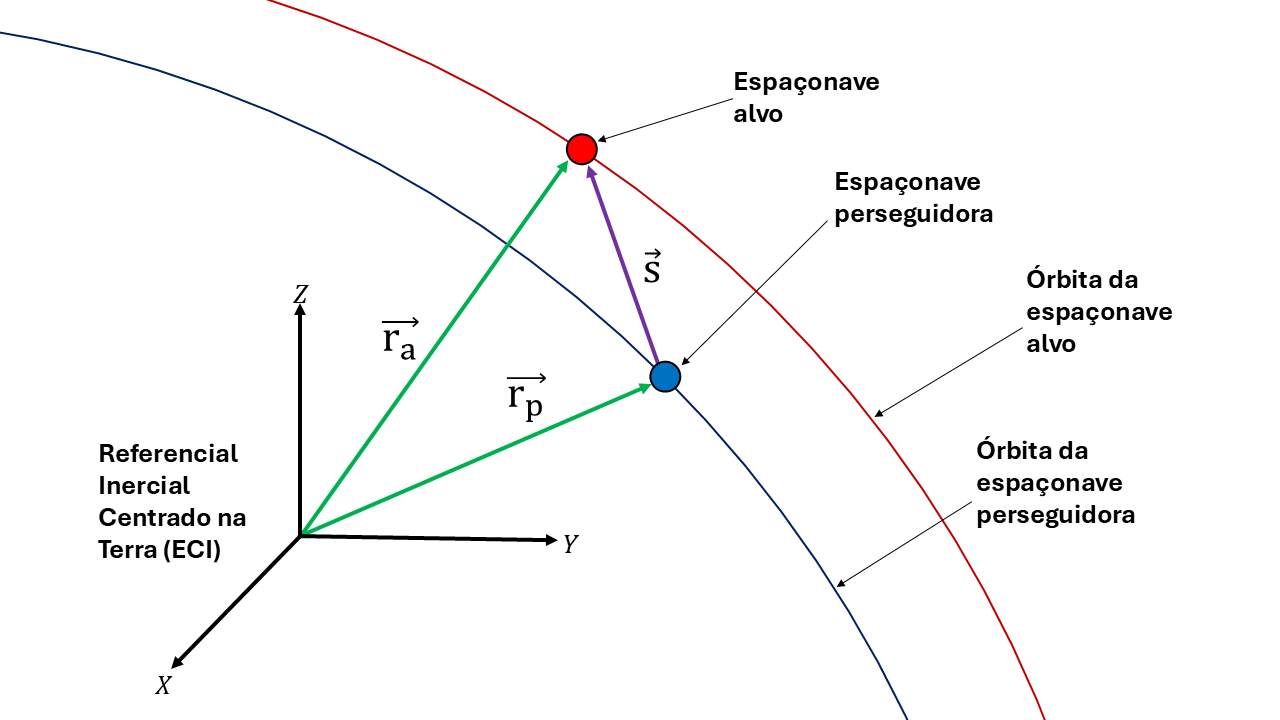
\includegraphics[width=1\linewidth]{4 Formulacao matematica/Imagens/Posicao absoluta.png}
\caption{Movimento relativo formulado para missões de \gls{rvdb} no referencial ECI.}
\label{fig:movimento_rvd_eci}
\end{figure}

A Figura~\ref{fig:movimento_rvd_eci} ilustra essa configuração para missões de \gls{rvdb}, em que o alvo e o perseguidor ocupam órbitas distintas em torno da Terra e o movimento relativo entre eles é definido a partir de suas posições no referencial inercial geocêntrico.


%%%%%%%%%%%%%%%%%%%%%%%% EQ MOV

% \section{Equações do Movimento Orbital e Manobras Associadas ao Problema de RVD/B}
\label{sec_eq_mov_orbital_manobras}

A formulação da dinâmica orbital no contexto de missões de RVD/B leva em consideração as diferentes fases da missão.
Quando o lançador atinge a altitude nominal, é realizada a injeção pelo perseguidor em órbita coplanar à órbita do alvo, órbita inicial, a $100$~km abaixo da órbita do alvo, que atenda condições orbitais estáveis para então iniciar as manobras de longa, curta e de proximidade subsequentes.

\subsection{Detalhes sobre a geometria da órbita do perseguidor}

Para que o veículo lançador insira a espaçonave perseguidora na órbita de injeção desejada, é necessário fornecer os elementos orbitais \cite{vallado2007fundamentals} de injeção ou o vetor posição--velocidade no referencial inercial (ECI) .
Neste trabalho foram considerados os elementos orbitais clássicos $(a, e, i, \Omega, \omega, M)$ e o vetor posição no referencial inercial no instante de injeção orbital.
Além disso, as condições para que a injeção orbital seja considerada válida incluem:

\begin{itemize}
    \item o correto posicionamento da altitude do lançador na altitude desejada;
    \item a fase orbital depende da janela de lançamento, podendo ser ajustada após a injeção e corrigida por espera, como no caso de deriva orbital.
\end{itemize}